\documentclass[10pt,a4paper]{article}
\usepackage[T1]{fontenc}
\usepackage[margin=2cm]{geometry}
\usepackage{isabelle,isabellesym}
\usepackage{amsmath,amssymb}
\usepackage{tikz}
\usetikzlibrary{calc,arrows.meta}
\usepackage{float}
\usepackage{pdfsetup}

\urlstyle{rm}
\isabellestyle{it}

\begin{document}

\title{Godsil's Path Tree and the Matching Polynomial}
\author{Carles Mar\'in}
\maketitle

\begin{abstract}
The path tree $T(G, u)$ of a finite graph $G$ at a vertex $u$ has one vertex for each simple path of $G$ that starts
at $u$, and joins each path to its one-step extensions. Godsil proved in 1981 that the matching polynomials of $G$
and of its path tree satisfy $\mu(G-u)\,\mu(T) = \mu(G)\,\mu(T-u)$, where $T - u$ removes the root, and that
$\mu(G)$ divides $\mu(T)$ when $G$ is connected. We formalize both statements, the second in the form that holds for
every graph: the matching polynomial of the connected component of $u$ divides $\mu(T)$. The entry builds on the
matching polynomial of the entry on the Heilmann--Lieb theorem.
\end{abstract}

\paragraph{Acknowledgement.} The formalization and the text of this document were prepared with the
assistance of an AI system, and checked by the author.

\tableofcontents

\section*{Introduction}

The matching polynomial $\mu(G, x) = \sum_M (-1)^{|M|} x^{n - 2|M|}$, the sum taken over all matchings $M$ of a graph
with $n$ vertices, has all its roots real by the theorem of Heilmann and Lieb~\cite{HeilmannLieb1972}. For a forest,
it equals the characteristic polynomial of the adjacency matrix~\cite{GodsilGutman1981}. Godsil~\cite{Godsil1981}
found a tree that carries the matching polynomial of any graph: the path tree. Its vertices are the simple paths that
start at a fixed vertex $u$, and a path is joined to every path obtained by adding one more vertex at its end
(Figure~\ref{fig:pathtree}). Godsil's theorem says that
\[
  \mu(G - u)\,\mu(T) = \mu(G)\,\mu(T - u), \qquad\text{and}\qquad \mu(G) \mid \mu(T) \text{ if $G$ is connected.}
\]
Since $\mu(T)$ is a characteristic polynomial of a symmetric matrix, the divisibility gives a second proof that the
roots of $\mu(G)$ are real; that consequence is not formalized here. A textbook account is in~\cite{Godsil1993}.

% generated by research/frisos-sturm/figura_godsil.py (Curiosity); do not edit by hand
\begin{figure}[H]
\centering
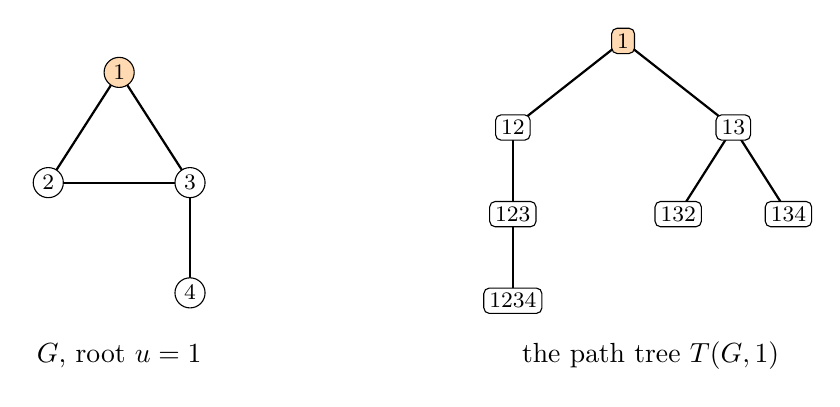
\begin{tikzpicture}[v/.style={circle, draw, fill=white, inner sep=1.5pt, font=\footnotesize}, t/.style={rounded corners=2pt, draw, fill=white, inner sep=2pt, font=\footnotesize}]
\begin{scope}[shift={(-4.2,-0.4)}]
  \draw[thick] (0.00,0.00) -- (-0.90,-1.40);
  \draw[thick] (0.00,0.00) -- (0.90,-1.40);
  \draw[thick] (-0.90,-1.40) -- (0.90,-1.40);
  \draw[thick] (0.90,-1.40) -- (0.90,-2.80);
  \node[v, fill=orange!30] at (0.00,0.00) {1};
  \node[v] at (-0.90,-1.40) {2};
  \node[v] at (0.90,-1.40) {3};
  \node[v] at (0.90,-2.80) {4};
  \node at (0,-3.6) {$G$, root $u = 1$};
\end{scope}
\begin{scope}[shift={(2.2,0)}]
  \draw[thick] (0.00,0.00) -- (-1.40,-1.10);
  \draw[thick] (0.00,0.00) -- (1.40,-1.10);
  \draw[thick] (1.40,-1.10) -- (0.70,-2.20);
  \draw[thick] (1.40,-1.10) -- (2.10,-2.20);
  \draw[thick] (-1.40,-1.10) -- (-1.40,-2.20);
  \draw[thick] (-1.40,-2.20) -- (-1.40,-3.30);
  \node[t, fill=orange!30] at (0.00,0.00) {1};
  \node[t] at (1.40,-1.10) {13};
  \node[t] at (2.10,-2.20) {134};
  \node[t] at (0.70,-2.20) {132};
  \node[t] at (-1.40,-1.10) {12};
  \node[t] at (-1.40,-2.20) {123};
  \node[t] at (-1.40,-3.30) {1234};
  \node at (0.35,-4.0) {the path tree $T(G, 1)$};
\end{scope}
\end{tikzpicture}
\caption{A graph and its path tree at vertex~1: one tree vertex for each path that starts at~1. Here $\mu(G) = x^{4} - 4 x^{2} + 1$ and $\mu(T) = x^{7} - 6 x^{5} + 9 x^{3} - 2 x = \mu(G)\,(x^{3} - 2 x)$.}
\label{fig:pathtree}
\end{figure}


The identity (theory \texttt{Path\_Tree}) is proved by induction on the number of vertices. Below its root, the path
tree of $G$ at $u$ is the disjoint union, over the neighbours $v$ of $u$, of the path trees of $G - u$ at $v$, up to
renaming each path by putting $u$ in front. So both sides of the identity can be computed with the vertex recurrence
of the matching polynomial at the root, the multiplicativity of $\mu$ on disjoint unions, and its invariance under
renaming.

The divisibility (theory \texttt{Path\_Tree\_Dvd}) needs connected components, which the identity does not see:
for a disconnected graph, $\mu(G)$ need not divide $\mu(T)$, since $T$ only sees the component of $u$. We define the
component of $u$ as the set of last vertices of the paths that start at $u$, and prove that the path trees of $G$ and
of this component at $u$ coincide. Removing $u$ from its component leaves the union of the components of its
neighbours in $G - u$. By induction, the matching polynomial of each of them divides the polynomial of the
corresponding branch of the tree, so $\mu(C - u)$ divides $\mu(T - u)$, and the identity applied to the component
$C$ gives $\mu(C) \mid \mu(T)$ after cancelling $\mu(C - u) \neq 0$. Figure~\ref{fig:roadmap} shows how the lemmas
fit together.

% Roadmap of the proof (names as in the theories).
\begin{figure}[H]
\centering
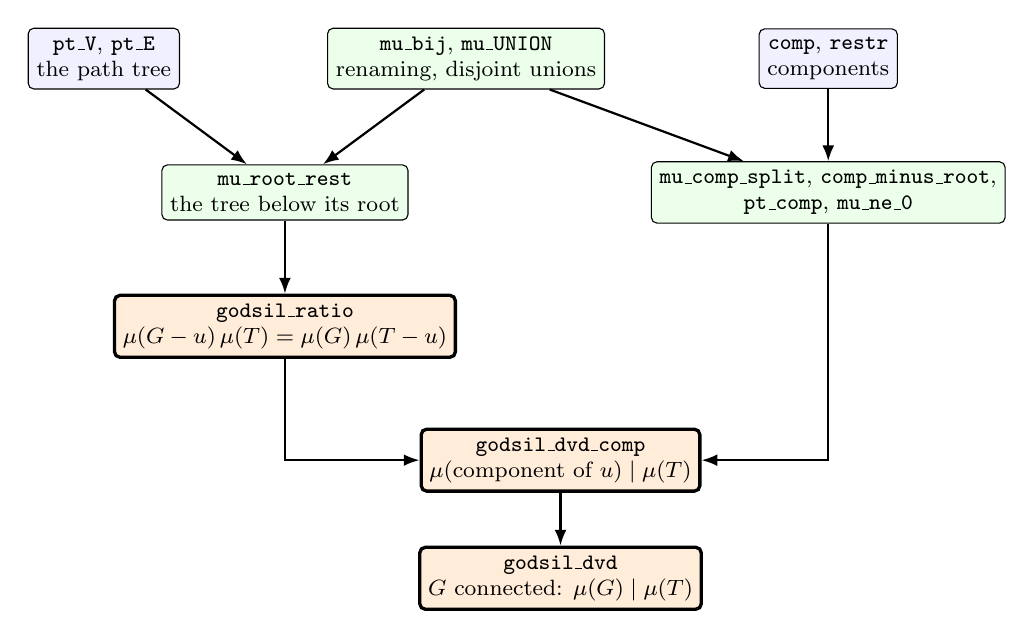
\begin{tikzpicture}[
    box/.style={draw, rounded corners=2pt, align=center, font=\footnotesize, inner sep=3pt, minimum height=7mm},
    def/.style={box, fill=blue!6},
    lem/.style={box, fill=green!8},
    thm/.style={box, fill=orange!15, very thick},
    arr/.style={-{Latex[length=2mm]}, thick}]
  \node[def] (pt)   at (-4.6,0)    {\texttt{pt\_V}, \texttt{pt\_E}\\ the path tree};
  \node[lem] (bij)  at (0,0)       {\texttt{mu\_bij}, \texttt{mu\_UNION}\\ renaming, disjoint unions};
  \node[def] (comp) at (4.6,0)     {\texttt{comp}, \texttt{restr}\\ components};
  \node[lem] (root) at (-2.3,-1.7) {\texttt{mu\_root\_rest}\\ the tree below its root};
  \node[thm] (rat)  at (-2.3,-3.4) {\texttt{godsil\_ratio}\\ $\mu(G-u)\,\mu(T) = \mu(G)\,\mu(T-u)$};
  \node[lem] (cl)   at (4.6,-1.7)  {\texttt{mu\_comp\_split}, \texttt{comp\_minus\_root},\\ \texttt{pt\_comp}, \texttt{mu\_ne\_0}};
  \node[thm] (dvd)  at (1.2,-5.1)  {\texttt{godsil\_dvd\_comp}\\ $\mu(\text{component of } u) \mid \mu(T)$};
  \node[thm] (cor)  at (1.2,-6.6)  {\texttt{godsil\_dvd}\\ $G$ connected: $\mu(G) \mid \mu(T)$};
  \draw[arr] (pt) -- (root);
  \draw[arr] (bij) -- (root);
  \draw[arr] (root) -- (rat);
  \draw[arr] (comp) -- (cl);
  \draw[arr] (bij) -- (cl);
  \draw[arr] (rat.south) |- (dvd.west);
  \draw[arr] (cl.south) |- (dvd.east);
  \draw[arr] (dvd) -- (cor);
\end{tikzpicture}
\caption{How the main lemmas lead to the theorems. Blue: definitions; green: lemmas; orange: the main results.}
\label{fig:roadmap}
\end{figure}


\parindent 0pt\parskip 0.5ex

\input{session}

\bibliographystyle{abbrv}
\bibliography{root}

\end{document}
